\documentclass{ctexart}
\ctexset{
    section = {
        titleformat = \raggedright,
        name = {,、},
        number = \chinese{section}
    }
}

\usepackage[colorlinks=false, linkcolor=blue, citecolor=blue, urlcolor=blue]{hyperref}
\usepackage[a4paper,top=2.54cm,bottom=2.54cm,left=3.18cm,right=3.18cm]{geometry}
\usepackage{amsmath,amsfonts,amssymb,amsthm}
\usepackage{tikz}
\usepackage{multirow}
\usepackage{array}
\usepackage{fancyhdr}
\usepackage{lastpage}
\usepackage{tabularx}
\usepackage{graphicx}
\usepackage{caption}
\usepackage{pifont}  
\usepackage{xcolor}
\usepackage{listings}
\usepackage{enumitem}
\usepackage{tocloft}  % 如果还没有导入的话
\usepackage{eso-pic}

\AddToShipoutPictureFG{%
  \AtPageCenter{%
    \begin{tikzpicture}[remember picture,overlay]
      \node[opacity=0.1] at (0,0) {\includegraphics[width=0.9\paperwidth,height=0.5\paperheight,keepaspectratio]{sy.png}};
    \end{tikzpicture}%
  }%
}

\definecolor{lightpink}{RGB}{184,83,182}
\definecolor{codebg}{RGB}{245,245,245}
\definecolor{emphcolor}{RGB}{199,21,133}
\definecolor{important}{RGB}{220,20,60}
\definecolor{highlight}{RGB}{0,100,0}
\definecolor{sumregion}{RGB}{255,200,200}
\definecolor{currentcell}{RGB}{255,0,0}
\definecolor{highlightpink}{RGB}{255,0,180}
\definecolor{lightgray}{gray}{0.8}
\definecolor{commentcolor}{RGB}{0,128,0}
\definecolor{keywordcolor}{RGB}{0,0,139}
\definecolor{conceptcolor}{RGB}{139,0,139}
\definecolor{stepcolor}{RGB}{0,100,0}
\definecolor{keypoint}{RGB}{0,100,0}
\definecolor{warning}{RGB}{255,0,0}

\hypersetup{
    pdfborder={0 0 0}  % 去掉链接的边框
}

\lstset{
basicstyle=\ttfamily\small,
language=C++,
frame=single,
breaklines=true,
backgroundcolor=\color{codebg},
escapeinside=``,
commentstyle=\color{green!60!black},
keywordstyle=\color{blue},
stringstyle=\color{red},
rulecolor=\color{black},
framesep=5pt,
xleftmargin=10pt,
xrightmargin=10pt
}

\setlist[enumerate,1]{label=\arabic*., leftmargin=2em}
\setlist[enumerate,2]{label=(\arabic*), leftmargin=3em}
\setlist[enumerate,3]{label=\roman*, leftmargin=4em}

\pagestyle{fancy}
\fancyhf{}
\cfoot{解码未来AI教育 \quad 编程题解 \quad 第\thepage 页}
\renewcommand{\headrulewidth}{0pt}


\begin{document}



% 生成目录
% 设置目录格式
\renewcommand{\contentsname}{\centering\Huge\bfseries 目录}
\renewcommand{\cfttoctitlefont}{\hfill\Huge\bfseries}  % 目录标题字体
\renewcommand{\cftaftertoctitle}{\hfill\mbox{}}        % 确保标题居中
\renewcommand{\cftsecfont}{\Large\bfseries}            % 一级章节字体(增大)
\renewcommand{\cftsecpagefont}{\Large\bfseries}        % 一级章节页码字体(增大)
\renewcommand{\cftsubsecfont}{\large\bfseries}         % 二级章节字体(增大) 
\renewcommand{\cftsubsecpagefont}{\large\bfseries}     % 二级章节页码字体(增大)
\renewcommand{\cftsecdotsep}{\cftdotsep}               % 点状分隔符

% 调整目录间距
\setlength{\cftbeforesecskip}{25pt}                    % 增大章节间间距
\setlength{\cftbeforesubsecskip}{15pt}                 % 增大子章节间间距
\setlength{\cftaftertoctitleskip}{30pt}                % 增大目录标题后的间距

% 增加目录项之间的额外间距
\addtocontents{toc}{\setlength{\parskip}{7pt}}        % 段落间距
\addtocontents{toc}{\setlength{\itemsep}{5pt}}         % 项目间距
\tableofcontents
\thispagestyle{empty}  % 目录页不显示页脚

\newpage
\thispagestyle{empty}  % 空白页不显示页脚
\subsection*{}

\newpage
\setcounter{page}{1}  % 重置页码为1,从正文开始计算页码

\section{L1212 : 汉明距离 \ding{78}} 

\subsection*{题目描述}
汉明距离是指\textcolor{lightpink}{\textbf{两个整数对应二进制位不同的数量}}。

例如,如果 $x = 1$(二进制表示为 0001),$y = 4$(二进制表示为 0100),那么它们的汉明距离是 2。

\subsection*{输入输出格式}
\textbf{输入:}一行两个数 $x$ $y$,表示需要计算的两个整数。其中($0 \leq x,y \leq 2^{30}$)\par
\textbf{输出:}$x$ 和 $y$ 的汉明距离。


\vspace{18pt}
\begin{table}[h]
\centering
\begin{tabularx}{\textwidth}{|X|X|}
\hline
\textbf{输入示例} & \textbf{输出示例}     \\    
\hline
1 4 & 2   \\ 
\hline
\end{tabularx}  
\end{table}

\subsection*{样例解释}
\begin{center}
$x = 1_{10} = 0001_2$ \\
$y = 4_{10} = 0100_2$
\end{center}

在二进制下,$x$ 和 $y$ 的表示如下:

\begin{table}[h]
\centering
\begin{tabularx}{0.9\textwidth}{|X|X|X|X|}
\hline
\textbf{位数} & \textbf{x} & \textbf{y} & \textbf{是否相同} \\   
\hline
第1位 & 1 & 0 & \textcolor{red}{不同} \\
\hline
第2位 & 0 & 0 & \textcolor{green!60!black}{相同} \\
\hline
第3位 & 0 & 1 & \textcolor{red}{不同} \\
\hline
第4位 & 0 & 0 & \textcolor{green!60!black}{相同} \\
\hline
\end{tabularx}  
\end{table}

$x$ 和 $y$ 二进制下有两处不同,所以汉明距离为 2。

\subsection*{背景知识}
位运算是对整数在二进制表示下直接对位进行的操作:
\begin{itemize}
\item \textbf{按位与(\&)}:两位都为1时结果为1
\item \textbf{按位或($|$)}:两位至少有一个为1时结果为1  
\item \textbf{按位异或(\^{} / $\oplus$)}:两位不同时结果为1,相同时结果为0
\item \textbf{左移($<<$)}:将所有位向左移动,右边补0
\item \textbf{右移($>>$)}:将所有位向右移动,左边补0
\end{itemize}

\subsection*{算法分析 : 使用位运算计算汉明距离}
\begin{enumerate}
\item \textbf{使用异或运算找出不同位}\\
使用\textcolor{lightpink}{异或($\oplus$)}运算的特性:相同为0,不同为1\\
计算 $x \oplus y$,使得 $x$ 和 $y$ 不同的部分标记为1,相同的部分标记为0。
\begin{lstlisting}
int t = x ^ y; `// 计算异或结果`
\end{lstlisting}

\item \textbf{使用与运算检查最后一位}\\
使用 \textcolor{lightpink}{\&} 运算判断最后一位是否为1:\\
对于 $( t \hspace{4pt} \& \hspace{4pt} 1 )$,如果值为1,则说明二进制下的 $t$ 在最后一位是1(因为只有 1\&1 = 1)。\\
如果值为0,则说明二进制下的 $t$ 在最后一位是0。
\begin{lstlisting}
cnt += t & 1; `// 检查最后一位是否为1`
\end{lstlisting}

\item \textbf{使用右移运算逐位处理}\\
使用\textcolor{lightpink}{右移($>>$)}运算逐位统计1的个数:\\
通过循环处理最后一位,如果是1(意味着此处 $x$ 和 $y$ 不同)则计数器加1,\\
然后将数字右移一位,直到数字变为0。
\end{enumerate}

\vspace{15pt}

\noindent\textbf{\large 示例:计算 $x=1$, $y=4$ 的汉明距离}
\begin{itemize}
\item \textbf{计算 $x \oplus y$}:
\begin{center}
$x = 1_{10} = 0001_2$ \\
$y = 4_{10} = 0100_2$ \\
$x \oplus y = 0101_2$
\end{center}

\item \textbf{统计 $x \oplus y$ 中1的个数}:
\vspace{10pt}
\begin{table}[h]
\centering
\begin{tabularx}{0.95\textwidth}{|>{\centering\arraybackslash}X|>{\centering\arraybackslash}X|>{\centering\arraybackslash}X|}
\hline
\textbf{当前目标值} & \textbf{最后一位数值} & \textbf{计数器数值} \\    
\hline 
0101 & 1(\textcolor{red}{$x$ 和 $y$ 不同}) & 1 \\ 
\hline
010 & 0(\textcolor{green!60!black}{$x$ 和 $y$ 相同}) & 1 \\ 
\hline
01 & 1(\textcolor{red}{$x$ 和 $y$ 不同}) & 2 \\ 
\hline
0 & 0(\textcolor{green!60!black}{$x$ 和 $y$ 相同}) & 2 \\ 
\hline
\end{tabularx}  
\end{table}
\end{itemize}

\subsection*{核心代码总览}
\begin{lstlisting}
int t = x ^ y; `// 计算异或结果`
int cnt = 0;   `//  计数器`
while (t) {    `// 当目标值为0时终止`
    cnt += t & 1; `// 检查最后一位是否为1`
    t >>= 1;      `// 右移一位`
}
\end{lstlisting}
\newpage

%%%%%%%%%%%%%%%%%%%%%%%%%%%%%%%%%%%%%%%%%%%%%%%%%%%%%%%%%%%%%%%%%%%%%%%%%%%%%%%%%%
%%%%%%%%%%%%%%%%%%%%%%%%%%%%%%%%%%%%%%%%%%%%%%%%%%%%%%%%%%%%%%%%%%%%%%%%%%%%%%%%%%
%%%%%%%%%%%%%%%%%%%%%%%%%%%%%%%%%%%%%%%%%%%%%%%%%%%%%%%%%%%%%%%%%%%%%%%%%%%%%%%%%%
%%%%%%%%%%%%%%%%%%%%%%%%%%%%%%%%%%%%%%%%%%%%%%%%%%%%%%%%%%%%%%%%%%%%%%%%%%%%%%%%%%
%%%%%%%%%%%%%%%%%%%%%%%%%%%%%%%%%%%%%%%%%%%%%%%%%%%%%%%%%%%%%%%%%%%%%%%%%%%%%%%%%%
%%%%%%%%%%%%%%%%%%%%%%%%%%%%%%%%%%%%%%%%%%%%%%%%%%%%%%%%%%%%%%%%%%%%%%%%%%%%%%%%%%
%%%%%%%%%%%%%%%%%%%%%%%%%%%%%%%%%%%%%%%%%%%%%%%%%%%%%%%%%%%%%%%%%%%%%%%%%%%%%%%%%%
%%%%%%%%%%%%%%%%%%%%%%%%%%%%%%%%%%%%%%%%%%%%%%%%%%%%%%%%%%%%%%%%%%%%%%%%%%%%%%%%%%



\section{L1507 : 值日 \ding{78}} 

\subsection*{题目描述}
小杨和小红是值日生,负责打扫教室。\textcolor{emphcolor}{\textbf{小杨每 $m$ 天值日一次}},\textcolor{emphcolor}{\textbf{小红每 $n$ 天值日一次}}。
今天他们两个一起值日,请问至少多少天后,他们会再次同一天值日?

\subsection*{输入输出格式}
\textbf{输入:}第一行,一个正整数 $m$,表示小杨的值日周期;\par
\qquad\quad 第二行,一个正整数 $n$,表示小红的值日周期。\par
\textbf{输出:}一行,一个整数,表示至少多少天后他们会再次同一天值日。

\begin{table}[h]
\centering
\begin{tabularx}{\textwidth}{|X|X|}
\hline
\textbf{输入示例} & \textbf{输出示例}     \\    
\hline
2 & 6   \\ 
3 & \\ 
\hline
\end{tabularx}  
\end{table}

\subsection*{样例解释}
小杨的值日周期 $m = 2$,小红的值日周期 $n = 3$。

从第0天开始,他们各自的值日安排如下表所示:
\begin{table}[h]
\centering
\begin{tabularx}{0.9\textwidth}{|c|*{7}{>{\centering\arraybackslash}X|}}
\hline
\textbf{天数} & 0 & 1 & 2 & 3 & 4 & 5 & 6 \\ 
\hline
小杨 & \textcolor{lightpink}{\textbf{是}} & 否 & \textcolor{lightpink}{\textbf{是}} & 否 & \textcolor{lightpink}{\textbf{是}} & 否 & \textcolor{lightpink}{\textbf{是}} \\ 
\hline
小红 & \textcolor{lightpink}{\textbf{是}} & 否 & 否 & \textcolor{lightpink}{\textbf{是}} & 否 & 否 & \textcolor{lightpink}{\textbf{是}} \\ 
\hline
\end{tabularx}  
\end{table}

从表中可以看出,他们下一次同时值日是第6天,输出结果为6。

\subsection*{背景知识}
\begin{itemize}
\item \textcolor{highlight}{\textbf{最小公倍数(LCM)}}:两个或多个整数公有的倍数中最小的一个。例如,2和3的最小公倍数是6($\text{LCM}(2,3) = 6$),4和8的最小公倍数是8($\text{LCM}(4,8) = 8$)。

\item \textcolor{highlight}{\textbf{最大公约数(GCD)}}:两个或多个整数共有约数中最大的一个。例如,2和3的最大公约数是1($\text{GCD}(2,3) = 1$),12和18的最大公约数是6($\text{GCD}(12,18) = 6$)。

\item \textcolor{highlight}{\textbf{重要关系}}:两个整数的最小公倍数与最大公约数满足:$$\text{GCD}(m, n) \times \text{LCM}(m, n) = m \times n$$
\end{itemize}

\subsection*{算法分析}
\begin{enumerate}
\item \textcolor{important}{\textbf{问题转化}}\\
小杨值日的日期是 $0, m, 2m, 3m, \ldots$,小红值日的日期是 $0, n, 2n, 3n, \ldots$。
因此,小杨和小红再次同一天值日的天数必须\textcolor{emphcolor}{\textbf{既是 $m$ 的倍数,又是 $n$ 的倍数}},从而得出最早的一天就是$m$ 和 $n$ 的\textcolor{important}{\textbf{最小公倍数}}($\text{LCM}(m,n)$)。

\newpage

\item \textcolor{important}{\textbf{计算$\text{LCM}(m,n)$}}
 \begin{enumerate}
    \item 使用 \_\_gcd() 计算 $\text{GCD}(m,n)$ 
    \item 通过最小公倍数和最大公约数关系($\text{GCD} \times \text{LCM}= m \times n$)计算 $\text{LCM}(m,n)$
 \end{enumerate}

\begin{lstlisting}
int GCD = __gcd(n, m);
int LCM = m * n / GCD;
\end{lstlisting}

\item \textcolor{important}{\textbf{欧几里得算法计算$\text{GCD}(m,n)$}}

\textbf{证明:$\text{GCD}(m, n)  = \text{GCD}(n, m \% n)$}
\begin{enumerate}
\item \textbf{基本情况}\\
假设 $m > n$,如果 $m$ 能被 $n$ 整除,那么 $\text{GCD}(m,n) = n$。
\item \textcolor{important}{\textbf{递推关系}}\\
如果 $m$ 不能被 $n$ 整除,我们可以得到关系式:$m = n \times k + r \quad (0 < r < n)$\par
其中:$k$ 是 $m \div n$ 的商,$r$ 是余数。\\
例如:$m = 16, n = 6$ 时,$16 = 6 \times 2 + 4$,所以 $k = 2, r = 4$。
\item \textcolor{important}{\textbf{关键证明}}\\
设 $d = \text{GCD}(m, n)$,则:
$d$ 能整除 $m$ 和 $n$,因此 $d$ 也能整除 $m - n \times k = r$,\par 所以 $d$ 是 $n$ 和 $r$ 的公约数。\par
因此我们得到:$d = \text{GCD}(m, n) = \text{GCD}(n, r) = \text{GCD}(n, m \% n)$
\end{enumerate}

\textbf{算法步骤:}

\begin{enumerate}
\item 计算 $\text{GCD}(m,n)$,当 $n \neq 0$ 时,重复以下步骤:
  \begin{enumerate}
  \item 计算余数 $r = m \% n$,令 $m = n$,$n = r$
  \item 当 $n = 0$ 时,$m$ 即为最大公约数
  \end{enumerate}
\end{enumerate}

\textbf{代码实现:}
    \begin{lstlisting}
while (n != 0) {
    int r = m % n;
    m = n;
    n = r;
}
return m;
    \end{lstlisting}

\textbf{示例:计算 $\text{GCD}(48, 18)$}

\begin{enumerate}[label={}, leftmargin=2em]
\item \textcolor{highlight}{\textbf{第一步}}:$48 \div 18 = 2$……$12$,所以 $\text{GCD}(48, 18) = \text{GCD}(18, 12)$
\item \textcolor{highlight}{\textbf{第二步}}:$18 \div 12 = 1$……$6$,所以 $\text{GCD}(18, 12) = \text{GCD}(12, 6)$  
\item \textcolor{highlight}{\textbf{第三步}}:$12 \div 6 = 2$……$0$,余数出现0,程序终止,所以 $\text{GCD}(12, 6) = 6$
\item \textcolor{important}{\textbf{最终结果}}:$\text{GCD}(48, 18) = 6$
\end{enumerate}


\end{enumerate}

\subsection*{拓展思考}
\begin{itemize}
    \item \textcolor{important}{\textbf{整数溢出问题}}:如果 $n$ 和 $m$ 很大,直接计算 $m \times n$ 可能会导致整数溢出。
    \item \textcolor{important}{\textbf{多人情况}}:如果是3个人、4个人,甚至是10000个人求下次同时值日的天数。
\end{itemize}
\newpage


%%%%%%%%%%%%%%%%%%%%%%%%%%%%%%%%%%%%%%%%%%%%%%%%%%%%%%%%%%%%%%%%%%%%%%%%%%%%%%%%%%
%%%%%%%%%%%%%%%%%%%%%%%%%%%%%%%%%%%%%%%%%%%%%%%%%%%%%%%%%%%%%%%%%%%%%%%%%%%%%%%%%%
%%%%%%%%%%%%%%%%%%%%%%%%%%%%%%%%%%%%%%%%%%%%%%%%%%%%%%%%%%%%%%%%%%%%%%%%%%%%%%%%%%
%%%%%%%%%%%%%%%%%%%%%%%%%%%%%%%%%%%%%%%%%%%%%%%%%%%%%%%%%%%%%%%%%%%%%%%%%%%%%%%%%%
%%%%%%%%%%%%%%%%%%%%%%%%%%%%%%%%%%%%%%%%%%%%%%%%%%%%%%%%%%%%%%%%%%%%%%%%%%%%%%%%%%
%%%%%%%%%%%%%%%%%%%%%%%%%%%%%%%%%%%%%%%%%%%%%%%%%%%%%%%%%%%%%%%%%%%%%%%%%%%%%%%%%%
%%%%%%%%%%%%%%%%%%%%%%%%%%%%%%%%%%%%%%%%%%%%%%%%%%%%%%%%%%%%%%%%%%%%%%%%%%%%%%%%%%
%%%%%%%%%%%%%%%%%%%%%%%%%%%%%%%%%%%%%%%%%%%%%%%%%%%%%%%%%%%%%%%%%%%%%%%%%%%%%%%%%%



\section{L1055 : 合并水果 \ding{78}\ding{78}} 

\subsection*{题目描述}
在一个果园里,张力恒同学已经将所有的果子打了下来,而且按果子的不同种类分成了不同的堆。
张力恒决定把所有的果子合成一堆。

每一次合并,张力恒可以把两堆果子合并到一起,消耗的体力等于两堆果子的重量之和。
可以看出,所有的果子经过 $n-1$ 次合并之后,就只剩下一堆了。张力恒在合并果子时总共消耗的体力等于每次合并所耗体力之和。

因为还要花大力气把这些果子搬回家,所以张力恒在合并果子时要尽可能地节省体力。
假定每个果子重量都为 1,并且已知果子的种类数和每种果子的数目,你的任务是设计出合并的次序方案,使多多耗费的体力最少,并输出这个最小的体力耗费值。

\subsection*{输入输出格式}
\textbf{输入:}第一行,一个整数 $n(1 \leq n \leq 10000)$,表示果子的种类数;  
第二行,包含 $n$ 个整数,用空格分隔,第 $i$ 个整数 $a_i(1 \leq a_i \leq 20000)$,
表示第 $i$ 种果子的数目。  
\textbf{输出:}一个整数,也就是最小的体力耗费值。输入数据保证这个值小于 $2^{31}$。

\vspace{6pt}
\begin{table}[h]
\centering
\begin{tabularx}{0.85\textwidth}{|X|X|}
\hline
\textbf{输入示例} & \textbf{输出示例}     \\    
\hline
3 & 15   \\ 
1 2 9 & \\ 
\hline
\end{tabularx}  
\end{table}

\subsection*{样例解释}
\begin{table}[h]
\centering
\renewcommand{\arraystretch}{0.8}
\begin{tabularx}{0.95\textwidth}{|c|>{\centering\arraybackslash}X|>{\centering\arraybackslash}X|>{\centering\arraybackslash}X|>{\centering\arraybackslash}X|}
\hline
\textbf{步骤} & \textbf{当前果堆状态} & \textbf{合并的果堆} & \textbf{本次消耗体力} & \textbf{累计消耗体力} \\ 
\hline
初始状态 & 1, 2, 9 & - & 0 & 0 \\ 
\hline
第一步 & 1, 2, 9 & 1 + 2 = 3 & 3 & 3 \\ 
\hline
第二步 & 3, 9 & 3 + 9 = 12 & 12 & 15 \\ 
\hline
\end{tabularx}  
\end{table}

\subsection*{算法分析}
\begin{enumerate}
\item \textbf{问题分析} \\ 
要使\textcolor{highlightpink}{总体力消耗最小},每次需要合并重量\textcolor{highlightpink}{最小}的两堆果子,重量小的果子被合并次数多,重量大的果子被合并次数少,总体力消耗最小。

\item \textbf{算法选择}
\begin{enumerate}
\item \textbf{朴素思想 : }  
每次从果堆中选出\textcolor{highlightpink}{最小}的两堆进行合并,再将合并后的重量插入数组并\textcolor{highlightpink}{重新排序},
重复操作直到只剩一堆。
每次排序花费时间为 $O(n \log n)$ , 一共进行 $n - 1$ 次合并,
所以总体时间复杂度为 $O(n^2 \log n)$ ,无法在 $1s$ 内执行完。

\item \textbf{使用优先队列 (\textcolor{blue}{priority\_queue}) 优化 : }  
使用\textcolor{blue}{最小堆}维护\textcolor{highlightpink}{最小元素},每次取出和插入元素均 $O(\log n)$,一共进行 $n - 1$ 次取出和插入,
因此总体复杂度 $O(n \log n)$ ,可以在 $1s$ 内执行完毕。

\item \textbf{实现思路}
\begin{itemize}
\setlength{\itemsep}{1pt}
\setlength{\parskip}{0pt}
\item 将所有果堆的{重量}放入\textcolor{blue}{最小堆}中
\item 每次取出两个\textcolor{highlightpink}{最小}元素,{合并}并累加\textcolor{highlightpink}{体力消耗}
\item 将合并后的{新堆重量}放回堆中,重复直到堆只剩一个元素
\end{itemize}
\end{enumerate}
\end{enumerate}

\subsection*{背景知识}
\begin{itemize}
    \item \textbf{\textcolor{blue}{优先队列(堆)}}:一种特殊的数据结构,可以快速获取和删除\textcolor{highlightpink}{最小(或最大)元素}。
\begin{lstlisting}
priority_queue<int, vector<int>, greater<int>> pq;
\end{lstlisting}

\begin{itemize}
  \setlength{\itemsep}{2pt} 
  \setlength{\parskip}{0pt}

  \item \textbf{\textcolor{blue}{第一个参数 \texttt{int}}}:指定队列中存储的元素类型
  \item \textbf{\textcolor{blue}{第二个参数 \texttt{vector<int>}}}:指定底层使用的容器,通常是vector
  \item \textbf{\textcolor{blue}{第三个参数 \texttt{greater<int>}}}:比较函数,决定元素的排列顺序
    \begin{itemize}
      \setlength{\itemsep}{1pt} 
      \setlength{\parskip}{0pt}
      \item \textcolor{highlightpink}{\texttt{less<int>}}:\textcolor{blue}{最大堆},最大的元素在顶部(默认值)
      \item \textcolor{highlightpink}{\texttt{greater<int>}}:\textcolor{blue}{最小堆},最小的元素在顶部
    \end{itemize}
\end{itemize}

\textbf{常用操作:}

\begin{table}[h]
\centering
\renewcommand{\arraystretch}{1.3}
\setlength{\tabcolsep}{10pt}
\begin{tabularx}{0.95\textwidth}{>{\centering\arraybackslash}p{3cm}|X|>{\centering\arraybackslash}p{2.5cm}}
\textbf{操作} & \textbf{功能说明} & \textbf{时间复杂度} \\
\hline
\texttt{pq.push(x)} & 将元素 \texttt{x} 插入堆 & $O(\log n)$ \\
\hline
\texttt{pq.pop()} & 删除堆顶部(最小或最大)元素 & $O(\log n)$ \\
\hline
\texttt{pq.top()} & 获取堆顶部元素 & $O(1)$ \\
\hline
\texttt{pq.empty()} & 判断堆是否为空 & $O(1)$ \\
\hline
\texttt{pq.size()} & 获取堆中元素个数 & $O(1)$ \\
\hline
\end{tabularx}
\end{table}
\end{itemize}



\subsection*{核心代码}
\begin{lstlisting}
while (pq.size() >= 2) { `// 重复操作直到堆中只剩一个元素`
    int u = pq.top();
    pq.pop();
    int v = pq.top();
    pq.pop();
    cnt += u + v; `// 取出两个最小的元素,合并它们,并累加体力消耗`
    pq.push(u + v); `// 合并结果放回堆中`
}
\end{lstlisting}

\subsection*{拓展思考}
\begin{itemize}
\item 如果每次合并三堆、四堆,甚至 k($k \leq 10^5$) 堆果子,算法该如何修改?
\item 如果要求改成求消耗体力的\textcolor{highlightpink}{最大值},该如何实现?
\end{itemize}
\newpage


%%%%%%%%%%%%%%%%%%%%%%%%%%%%%%%%%%%%%%%%%%%%%%%%%%%%%%%%%%%%%%%%%%%%%%%%%%%%%%%%%%
%%%%%%%%%%%%%%%%%%%%%%%%%%%%%%%%%%%%%%%%%%%%%%%%%%%%%%%%%%%%%%%%%%%%%%%%%%%%%%%%%%
%%%%%%%%%%%%%%%%%%%%%%%%%%%%%%%%%%%%%%%%%%%%%%%%%%%%%%%%%%%%%%%%%%%%%%%%%%%%%%%%%%
%%%%%%%%%%%%%%%%%%%%%%%%%%%%%%%%%%%%%%%%%%%%%%%%%%%%%%%%%%%%%%%%%%%%%%%%%%%%%%%%%%
%%%%%%%%%%%%%%%%%%%%%%%%%%%%%%%%%%%%%%%%%%%%%%%%%%%%%%%%%%%%%%%%%%%%%%%%%%%%%%%%%%
%%%%%%%%%%%%%%%%%%%%%%%%%%%%%%%%%%%%%%%%%%%%%%%%%%%%%%%%%%%%%%%%%%%%%%%%%%%%%%%%%%
%%%%%%%%%%%%%%%%%%%%%%%%%%%%%%%%%%%%%%%%%%%%%%%%%%%%%%%%%%%%%%%%%%%%%%%%%%%%%%%%%%
%%%%%%%%%%%%%%%%%%%%%%%%%%%%%%%%%%%%%%%%%%%%%%%%%%%%%%%%%%%%%%%%%%%%%%%%%%%%%%%%%%



\section{L1530 : 二维数组前缀和 \ding{78}\ding{78}} 

\subsection*{题目描述}
给定一个 $n$ 行 $m$ 列的二维数组,你需要计算该数组的\textcolor{emphcolor}{\textbf{前缀和}}。

所谓前缀和是指:对于每个位置 $(i,j)$,求出从左上角 $(0,0)$ 到当前位置 $(i,j)$ 的所有元素的和。

\[
a = 
\begin{bmatrix}
1 & 2 & 3\\
4 & 5 & 6\\
7 & 8 & 9
\end{bmatrix}
\quad\Rightarrow\quad
s =
\begin{bmatrix}
1 & 3 & 6\\
5 & 12 & 21\\
12 & 27 & 45
\end{bmatrix}
\]

\subsection*{输入输出格式}
\textbf{输入:}第一行包含两个整数 $n, m$($1 \le n, m \le 1000$),表示二维数组的行数和列数。\par
\qquad\quad 接下来的 $n$ 行,每行包含 $m$ 个整数,表示二维数组的元素。\par
\qquad\quad 每个元素的值满足 $-10^3 \le a[i][j] \le 10^3$。\par
\textbf{输出:}输出 $n$ 行,每行包含 $m$ 个整数,表示前缀和数组对应位置的值。\par
\qquad\quad 每行数之间用一个空格分隔,且\textcolor{red}{每行末尾不要有空格}。

\begin{table}[h]
\centering
\begin{tabularx}{\textwidth}{|X|X|}
\hline
\textbf{输入示例} & \textbf{输出示例}     \\    
\hline
3 3 & 1 3 6 \\ 
1 2 3 & 5 12 21 \\ 
4 5 6 & 12 27 45 \\ 
7 8 9 & \\ 
\hline
\end{tabularx}  
\end{table}

\subsection*{样例解释}
以计算 $s[1][2]$(第二行第三列)为例,演示二维前缀和的计算过程:
\begin{align*}
s[1][2] &= a[0][0] + a[0][1] + a[0][2] + a[1][0] + a[1][1] + a[1][2] \\
&= 1 + 2 + 3 + 4 + 5 + 6 \\
&= 21
\end{align*}

\subsection*{算法分析}

\begin{enumerate}
\item \textcolor{highlight}{\textbf{直接计算方法}}\\
对于每个位置 $(i,j)$,直接计算从 $(0,0)$ 到 $(i,j)$ 的所有元素之和:
\begin{lstlisting}[language=C++]
for(int x = 0; x <= i; x++) {
    for(int y = 0; y <= j; y++) {
        s[i][j] += a[x][y];
    }
}   
\end{lstlisting}

这种方法的时间复杂度为 $O(n^2 \cdot m^2)$,会导致超时。

\item \textcolor{highlight}{\textbf{优化方法:前缀和}}\\
利用已计算的前缀和来计算新的前缀和,可以大大降低时间复杂度。以下以 $s[2][2]$ 的计算为例进行说明。

\begin{enumerate}
\item \textcolor{highlight}{\textbf{区域划分}}\\
我们用不同颜色表示不同的前缀和区域,$s[2][2]$ = 整个矩形内所有数字的和 :

\begin{center}
\begin{tabular}{ccc}
$\begin{bmatrix}
\textcolor{blue}{1} & \textcolor{blue}{2} & \textcolor{blue}{3}\\
\textcolor{blue}{4} & \textcolor{blue}{5} & \textcolor{blue}{6}\\
7 & 8 & \textcolor{orange}{9}
\end{bmatrix}$
&
$\begin{bmatrix}
\textcolor{red}{1} & \textcolor{red}{2} & 3\\
\textcolor{red}{4} & \textcolor{red}{5} & 6\\
\textcolor{red}{7} & \textcolor{red}{8} & \textcolor{orange}{9}
\end{bmatrix}$
&
$\begin{bmatrix}
\textcolor{green}{1} & \textcolor{green}{2} & 3\\
\textcolor{green}{4} & \textcolor{green}{5} & 6\\
7 & 8 & \textcolor{orange}{9}
\end{bmatrix}$
\end{tabular}
\end{center}

\begin{itemize}
\item 蓝色部分的数字和表示 $s[1][2]$,红色部分的数字和表示 $s[2][1]$,
绿色部分的数字和表示 $s[1][1]$(红蓝重叠的部分),橘色部分的数字表示 $a[2][2]$。
\item 整个矩形的和 = 蓝色区域 + 红色区域 - 绿色区域 + 橘色区域
\item 用符号表示就是: 
$s[2][2] = 
\textcolor{blue}{s[1][2]} + \textcolor{red}{s[2][1]} - 
\textcolor{green}{s[1][1]} + \textcolor{orange}{a[2][2]}$
\item 得出通用公式:$s[x][y] = 
\textcolor{blue}{s[x-1][y]} + \textcolor{red}{s[x][y-1]} - 
\textcolor{green}{s[x-1][y-1]} + \textcolor{orange}{a[x][y]}
$\\
当前位置前缀和 = \textcolor{blue}{左前缀和} + 
\textcolor{red}{上前缀和} - 
\textcolor{green}{左上角前缀和} + 
\textcolor{orange}{当前位置的值}
\item 我们利用这个公式,从左上角到右下角的顺序,计算$s[i][j]$,就可以得到所有 $s[x][y]$ 的值。
\end{itemize}
\end{enumerate}
\end{enumerate}

\subsection*{代码实现:}
\text{处理前缀和}
\begin{lstlisting}
for (int i = 1; i <= n; i++) {
    for (int j = 1; j <= m; j++) {
        s[i][j] += s[i - 1][j] + s[i][j - 1] - 
                   s[i - 1][j - 1] + a[i - 1][j - 1];
    }
}
\end{lstlisting}

\text{输出格式}
\begin{lstlisting}
`//注意行末不能有多余的空格`
for (int i = 0; i < n; i++) {
    for (int j = 0; j < m; j++) {
        cout << a[i][j] << "` `\n"[j == m - 1];
    }
}
\end{lstlisting}

\subsection*{拓展思考}
\begin{itemize}
    \item 如果换成三维,如何求 $a[i][j][k]$ 的前缀和?
    \item 如果要求从 $(x1,y1)$ 到 $(x2,y2)$ 的区域和,该如何计算?
\end{itemize}
\newpage



%%%%%%%%%%%%%%%%%%%%%%%%%%%%%%%%%%%%%%%%%%%%%%%%%%%%%%%%%%%%%%%%%%%%%%%%%%%%%%%%%%
%%%%%%%%%%%%%%%%%%%%%%%%%%%%%%%%%%%%%%%%%%%%%%%%%%%%%%%%%%%%%%%%%%%%%%%%%%%%%%%%%%
%%%%%%%%%%%%%%%%%%%%%%%%%%%%%%%%%%%%%%%%%%%%%%%%%%%%%%%%%%%%%%%%%%%%%%%%%%%%%%%%%%
%%%%%%%%%%%%%%%%%%%%%%%%%%%%%%%%%%%%%%%%%%%%%%%%%%%%%%%%%%%%%%%%%%%%%%%%%%%%%%%%%%
%%%%%%%%%%%%%%%%%%%%%%%%%%%%%%%%%%%%%%%%%%%%%%%%%%%%%%%%%%%%%%%%%%%%%%%%%%%%%%%%%%
%%%%%%%%%%%%%%%%%%%%%%%%%%%%%%%%%%%%%%%%%%%%%%%%%%%%%%%%%%%%%%%%%%%%%%%%%%%%%%%%%%
%%%%%%%%%%%%%%%%%%%%%%%%%%%%%%%%%%%%%%%%%%%%%%%%%%%%%%%%%%%%%%%%%%%%%%%%%%%%%%%%%%
%%%%%%%%%%%%%%%%%%%%%%%%%%%%%%%%%%%%%%%%%%%%%%%%%%%%%%%%%%%%%%%%%%%%%%%%%%%%%%%%%%




\section{L1424 : IP地址 \ding{78}\ding{78}} 

\subsection*{题目描述}
给定一个字符串 $s$,请你判断它是否是一个有效的 IPv4 地址。

一个有效的 IPv4 地址由四个整数构成,这些整数位于 0 到 255 之间,用 '.' 分隔。

每个整数不能有前导零(除非该整数本身就是 0),并且每个部分必须是非空的。

\subsection*{输入输出格式}
\textbf{输入:}输入包含多组测试数据。每组测试数据占一行,
包含一个字符串 $s$ ($1 \le |s| \le 15$)。 输入以文件结束符(EOF)结束。\par
\textbf{输出:}对于每组测试数据,如果输入的字符串 $s$ 是一个有效的 
IPv4 地址,则输出 "YES";否则输出 "NO"。每个输出占一行。

\begin{table}[h]
\centering
\begin{tabularx}{\textwidth}{|X|X|}
\hline
\textbf{输入示例} & \textbf{输出示例}     \\    
\hline
192.168.1.1 & YES \\ 
192.168.1.01 & NO \\ 
0.0.0.0 & YES \\ 
255.255.255.255 & YES \\ 
\hline
\end{tabularx}  
\end{table}

\subsection*{样例解释}
\begin{itemize}
\item \textbf{192.168.1.1}: 所有部分都在 0-255 范围内,没有前导零,格式正确,输出 YES
\item \textbf{192.168.1.01}: 第四部分 "01" 有前导零,不符合要求,输出 NO
\item \textbf{0.0.0.0}: 所有部分都是 0,允许单个 0,输出 YES
\item \textbf{255.255.255.255}: 所有部分都在 0-255 范围内,没有前导零,格式正确,输出 YES
\end{itemize}

\subsection*{算法分析}

\begin{enumerate}
\item \textcolor{highlight}{\textbf{验证条件}}
\begin{itemize}
\item 恰好包含 3 个点号 '.',分成 4 个部分
\item 每部分为 0-255 的整数且无前导零
\end{itemize}

\item \textcolor{highlight}{\textbf{实现思路}}
\begin{enumerate}
\item 按 '.' 分割字符串为 4 部分
\item 每部分是否都是数字 且 大小在 0-255 范围内
\item 无前导零
\end{enumerate}
\end{enumerate}

\subsection*{代码实现:}

\text{判断逻辑 : }
\begin{lstlisting}
bool check (string s) {
    if (s.size() > 3 || s.size() == 0) return false; 
    `//超出3位数,或者是空的 直接不满足[0,255]条件`
    for (int i = 0; i < s.size(); i++) {
        if (s[i] > '9' || s[i] < '0') return false;
        `//验证都是数字`
    }
    for (int i = 0; i < s.size(); i++) { `//验证无前导零`
        if (s[i] == '0' && s.size() > 1) {
            return false;`//除了"0"之外,字符串开头是0的都不合法`
        } else if (s.size() > 1) {
            break;
        }
    }
    
    int num = stoi(s); `//字符串转换为数字`
    if (num < 0 || num > 255) return false; `//判断是否在[0,255]范围内`
    return true;
};
\end{lstlisting}

\text{字符串处理 : }

\begin{lstlisting}
while (cin >> s) {
    string t;
    bool ok = true;
    for (int i = 0; i < s.size(); i++) {
        if (s[i] == '.') { ` // 遇到分割符号,检查当前部分是否满足要求`
            ok &= check(t);
            t.clear();
        } else {
            t += s[i];
        }
    }

    ok &= check(t); ` // 检查最后一部分`

    if (ok) {
        cout << "YES\n";
    } else {
        cout << "NO\n";
    }
}
\end{lstlisting}
\subsection*{拓展思考 :}
\begin{itemize}
\item 给定任意一个字符串和
一个分割的字符集,
如何实现一个通用的字符串分割函数?
\end{itemize}
\newpage


%%%%%%%%%%%%%%%%%%%%%%%%%%%%%%%%%%%%%%%%%%%%%%%%%%%%%%%%%%%%%%%%%%%%%%%%%%%%%%%%%%
%%%%%%%%%%%%%%%%%%%%%%%%%%%%%%%%%%%%%%%%%%%%%%%%%%%%%%%%%%%%%%%%%%%%%%%%%%%%%%%%%%
%%%%%%%%%%%%%%%%%%%%%%%%%%%%%%%%%%%%%%%%%%%%%%%%%%%%%%%%%%%%%%%%%%%%%%%%%%%%%%%%%%
%%%%%%%%%%%%%%%%%%%%%%%%%%%%%%%%%%%%%%%%%%%%%%%%%%%%%%%%%%%%%%%%%%%%%%%%%%%%%%%%%%
%%%%%%%%%%%%%%%%%%%%%%%%%%%%%%%%%%%%%%%%%%%%%%%%%%%%%%%%%%%%%%%%%%%%%%%%%%%%%%%%%%
%%%%%%%%%%%%%%%%%%%%%%%%%%%%%%%%%%%%%%%%%%%%%%%%%%%%%%%%%%%%%%%%%%%%%%%%%%%%%%%%%%
%%%%%%%%%%%%%%%%%%%%%%%%%%%%%%%%%%%%%%%%%%%%%%%%%%%%%%%%%%%%%%%%%%%%%%%%%%%%%%%%%%
%%%%%%%%%%%%%%%%%%%%%%%%%%%%%%%%%%%%%%%%%%%%%%%%%%%%%%%%%%%%%%%%%%%%%%%%%%%%%%%%%%





\section{L1426 : 学生统计 \ding{78}\ding{78}} 

\subsection*{题目描述}
快开学了,小徐同学想帮老师统计一下本学期学校的学生信息。

老师给了一张学生信息表,每一条数据包括学生姓名、年级、班级。

老师想知道本学期每个年级有多少个班以及多少个人。

\subsection*{输入输出格式}
\textbf{输入:}第一行,一个整数 $N$,表示有 $N$ 条数据;  
接下来 $N$ 行,每行包含三个字符串,分别表示姓名、年级、班级。  

\textbf{输出:}按年级从小到大,输出年级的班级数和总人数。  
(注意,年级、班级总数、年级总数之间有一个空格,每行末尾不要有空格)

\vspace{12pt}
\begin{table}[h]
\centering
\begin{tabularx}{0.85\textwidth}{|X|X|}
\hline
\textbf{输入示例} & \textbf{输出示例}     \\    
\hline
5 & G7 2 3   \\ 
Tom G7 A & G8 1 2   \\ 
Jerry G7 B & \\ 
Llice G7 A & \\ 
Bob G8 A & \\ 
Apple G8 A & \\ 
\hline
\end{tabularx}  
\end{table}

\subsection*{样例解释}
\begin{table}[h]
\centering
\begin{tabularx}{0.95\textwidth}{|c|>{\centering\arraybackslash}X|>{\centering\arraybackslash}X|>{\centering\arraybackslash}X|}
\hline
\textbf{年级} & \textbf{班级列表} & \textbf{班级数} & \textbf{学生人数} \\ 
\hline
G7 & A班:Tom、Llice \quad B班:Jerry & 2 & 3 \\ 
\hline
G8 & A班:Bob、Apple & 1 & 2 \\ 
\hline
\end{tabularx}  
\end{table}

\subsection*{算法分析}
\begin{enumerate}
\item \textbf{问题分析} \\ 
需要统计\textcolor{highlightpink}{每个年级的班级数}和\textcolor{highlightpink}{学生总数}。
同一个年级的不同班级需要去重统计,而同一个年级的学生人数直接累加。

\item \textbf{算法选择}
\begin{enumerate}
\item \textbf{\textcolor{highlight}{解法一 - 排序 + 遍历统计} : }  
先将所有学生信息按\textcolor{highlightpink}{年级}和
\textcolor{highlightpink}{班级}排序,
将年级小的放在前面,年级相同的按照班级排序,
然后遍历统计每个年级的信息。

\item \textbf{\textcolor{highlight}{解法二 - Map/Set 统计} : }  
使用 \texttt{map} 和 \texttt{set} 容器自动维护有序性和去重特性,将年级作为键,班级,学生人数作为值
\end{enumerate}

\item \textbf{实现思路}
\begin{itemize}
    \item \textbf{\textcolor{highlight}{法一}:结构体排序 + 遍历统计}
    \begin{enumerate}
\setlength{\itemsep}{1pt}
\setlength{\parskip}{0pt}
\item 定义结构体存储学生信息(姓名、年级、班级)
\begin{lstlisting}[language=C++]
struct Node {
    string g;
    string c;
    string n;
};

bool cmp(Node a, Node b) {
    if (a.g == b.g) return a.c < b.c;
    return a.g < b.g;
}
\end{lstlisting}
\item 按\textcolor{blue}{年级升序、班级升序}排序
\item 遍历排序后的数据,统计每个年级的班级数和学生数
\begin{lstlisting}[language=C++]
if (g != a[i].g) { `// 枚举到了新的年级`
    cout << g << "` `" << cnt_class << "` `" 
         << cnt_stu << endl;` // 先输出上一个年级的信息`
    g = a[i].g, c = a[i].c;
    cnt_class = 1, cnt_stu = 0;` // 数据清零`
}
cnt_stu++;
if (c != a[i].c) {` // 遇到新的班级,班级数加1`
    c = a[i].c;
    cnt_class++;
}
\end{lstlisting}
\end{enumerate}


\item \textbf{\textcolor{highlight}{法二}:map + set 统计}
\begin{enumerate}
\item 使用 \texttt{map<string, int>} 统计每个年级的学生总数
\begin{lstlisting}[language=C++]
map<string, int> s;` // 年级 -> 学生数`
s[grade]++;
\end{lstlisting}

\item 使用 \texttt{map<string, set<string>>} 统计每个年级的班级集合(自动去重)
\begin{lstlisting}[language=C++]
map<string, set<string>> c;` // 年级 -> 班级集合`
c[grade].insert(clazz);
\end{lstlisting}

\item 遍历 \texttt{map} 输出结果
\begin{lstlisting}[language=C++]
for (auto i : s) {
    cout << i.first << "` `" << c[i.first].size() << "` `" 
         << i.second << endl;
}
\end{lstlisting}


\end{enumerate}
\end{itemize}

\end{enumerate}




\subsection*{拓展思考}
\begin{itemize}
\item 如果要求按\textcolor{highlightpink}{班级数从大到小}输出,该如何修改排序规则?
\item 如果数据中存在重复记录(相同姓名、年级、班级),该如何去重?
\end{itemize}
\newpage

%%%%%%%%%%%%%%%%%%%%%%%%%%%%%%%%%%%%%%%%%%%%%%%%%%%%%%%%%%%%%%%%%%%%%%%%%%%%%%%%%%
%%%%%%%%%%%%%%%%%%%%%%%%%%%%%%%%%%%%%%%%%%%%%%%%%%%%%%%%%%%%%%%%%%%%%%%%%%%%%%%%%%
%%%%%%%%%%%%%%%%%%%%%%%%%%%%%%%%%%%%%%%%%%%%%%%%%%%%%%%%%%%%%%%%%%%%%%%%%%%%%%%%%%
%%%%%%%%%%%%%%%%%%%%%%%%%%%%%%%%%%%%%%%%%%%%%%%%%%%%%%%%%%%%%%%%%%%%%%%%%%%%%%%%%%
%%%%%%%%%%%%%%%%%%%%%%%%%%%%%%%%%%%%%%%%%%%%%%%%%%%%%%%%%%%%%%%%%%%%%%%%%%%%%%%%%%
%%%%%%%%%%%%%%%%%%%%%%%%%%%%%%%%%%%%%%%%%%%%%%%%%%%%%%%%%%%%%%%%%%%%%%%%%%%%%%%%%%
%%%%%%%%%%%%%%%%%%%%%%%%%%%%%%%%%%%%%%%%%%%%%%%%%%%%%%%%%%%%%%%%%%%%%%%%%%%%%%%%%%
%%%%%%%%%%%%%%%%%%%%%%%%%%%%%%%%%%%%%%%%%%%%%%%%%%%%%%%%%%%%%%%%%%%%%%%%%%%%%%%%%%


\section{L1491 : 字符串基础2 \ding{78}\ding{78}} 

\subsection*{题目描述}
一串长度不超过 255 的 PASCAL 语言代码,只有 \textcolor{keywordcolor}{a, b, c 三个变量},
而且只有\textcolor{keywordcolor}{赋值语句},赋值只能是一个\textcolor{keywordcolor}{一位的数字}或一个\textcolor{keywordcolor}{变量},
每条赋值语句的格式是 \textcolor{red}{[变量]:=[变量或一位整数];}。
\textcolor{keywordcolor}{未赋值的变量值为 0},输出 a, b, c 的值。

\subsection*{输入输出格式}
\textbf{输入:}一串符合语法的 PASCAL 语言代码,\textcolor{keywordcolor}{只有 a, b, c 三个变量},\par
\qquad\quad 而且\textcolor{keywordcolor}{只有赋值语句},赋值只能是一个\textcolor{keywordcolor}{一位的数字}或一个\textcolor{keywordcolor}{变量},\par 
\qquad\quad \textcolor{keywordcolor}{未赋值的变量值为 0}。\par
\textbf{输出:}输出 a, b, c 最终的值。\\[0.5em]

\begin{table}[h]
\centering
\begin{tabularx}{\textwidth}{|X|X|}
\hline
\textbf{输入示例} & \textbf{输出示例}     \\    
\hline
a:=3;b:=4;c:=5; & 3 4 5 \\ 
\hline
a:=3;b:=a;c:=a; & 3 3 3 \\ 
\hline
a:=3;b:=a; & 3 3 0 \\ 
\hline
\end{tabularx}  
\end{table}

\subsection*{样例解释}
\begin{enumerate}
\item \texttt{a:=3;b:=4;c:=5;}\\
变量 a 被赋值为 3,变量 b 被赋值为 4,变量 c 被赋值为 5,所以输出 \texttt{3 4 5}。

\item \texttt{a:=3;b:=a;c:=a;}\\
变量 a 被赋值为 3,变量 b 被赋值为 a 的值(3),变量 c 被赋值为 a 的值(3),所以输出 \texttt{3 3 3}。

\item \texttt{a:=3;b:=a;}\\
变量 a 被赋值为 3,变量 b 被赋值为 a 的值(3),变量 c 没有被赋值(保持初始值 0),所以输出 \texttt{3 3 0}。
\end{enumerate}

\subsection*{算法分析}

\begin{enumerate}
\item \textcolor{highlight}{\textbf{问题分析}}\\
本题需要\textcolor{conceptcolor}{提取字符串中有效的部分},并\textcolor{conceptcolor}{跟踪三个变量 a, b, c 的值变化}。
赋值语句的格式固定,可以\textcolor{conceptcolor}{按分号分割语句},然后逐个解析。

\item \textcolor{highlight}{\textbf{关键步骤}}
\begin{enumerate}
\item \textcolor{stepcolor}{\textbf{初始化变量:}} 创建三个变量 a, b, c,初始值都为 0。
\item \textcolor{stepcolor}{\textbf{分割语句:}} 将输入字符串按分号分割成多个赋值语句。
\item \textcolor{stepcolor}{\textbf{解析每条语句:}} 对于每条语句,提取左侧变量和右侧值。
\item \textcolor{stepcolor}{\textbf{赋值处理:}} 如果右侧是数字,直接赋值;如果右侧是变量,
则使用该字母对应的数值。
\item \textcolor{stepcolor}{\textbf{输出结果:}} 处理完所有语句后,输出 a, b, c 的最终值。
\end{enumerate}

\item \textcolor{highlight}{\textbf{字符串处理技巧}}
\begin{itemize}
\item 使用 \textcolor{conceptcolor}{$map<char,int>$ 记录字母对应的数值}(默认初始值为 0)。
\begin{lstlisting}
map<char, int> mp;
mp['a'] = 0; mp['b'] = 0; mp['c'] = 0;
\end{lstlisting}

\item 使用 $map<char,int>$ 将 \textcolor{conceptcolor}{字符(char 类型)和数字(int 类型)等价}。例如 $mp['1'] = 1$(前者是 $char$ 类型,后者是 $int$ 类型)。
\begin{lstlisting}
for (int i = 0; i < 10; i++) {
    mp['0' + i] = i;
}
\end{lstlisting}
\item 根据一个赋值语句 【$a:=3;$】 占据 5 个字符,
因此把\textcolor{conceptcolor}{5 个字符为一个完整的赋值语句}。
在每次循环中,$a$ 是在0位置,$b$ 是在3位置, 所以只需要将 $mp[s[0]]$ 赋值为 $mp[s[3]]$ 即可。
\begin{lstlisting}
for (int i = 0; i < s.size(); i += 5) {
    mp[s[i]] = mp[s[i + 3]];
}
\end{lstlisting}
\end{itemize}
\end{enumerate}


\subsection*{拓展思考}
\begin{itemize}
    \item 如果\textcolor{conceptcolor}{变量名不止 a, b, c 三个},如何扩展程序?
    \item 如果\textcolor{conceptcolor}{赋值语句不止 3 句},如何处理?
\end{itemize}
\newpage



%%%%%%%%%%%%%%%%%%%%%%%%%%%%%%%%%%%%%%%%%%%%%%%%%%%%%%%%%%%%%%%%%%%%%%%%%%%%%%%%%%
%%%%%%%%%%%%%%%%%%%%%%%%%%%%%%%%%%%%%%%%%%%%%%%%%%%%%%%%%%%%%%%%%%%%%%%%%%%%%%%%%%
%%%%%%%%%%%%%%%%%%%%%%%%%%%%%%%%%%%%%%%%%%%%%%%%%%%%%%%%%%%%%%%%%%%%%%%%%%%%%%%%%%
%%%%%%%%%%%%%%%%%%%%%%%%%%%%%%%%%%%%%%%%%%%%%%%%%%%%%%%%%%%%%%%%%%%%%%%%%%%%%%%%%%
%%%%%%%%%%%%%%%%%%%%%%%%%%%%%%%%%%%%%%%%%%%%%%%%%%%%%%%%%%%%%%%%%%%%%%%%%%%%%%%%%%
%%%%%%%%%%%%%%%%%%%%%%%%%%%%%%%%%%%%%%%%%%%%%%%%%%%%%%%%%%%%%%%%%%%%%%%%%%%%%%%%%%
%%%%%%%%%%%%%%%%%%%%%%%%%%%%%%%%%%%%%%%%%%%%%%%%%%%%%%%%%%%%%%%%%%%%%%%%%%%%%%%%%%
%%%%%%%%%%%%%%%%%%%%%%%%%%%%%%%%%%%%%%%%%%%%%%%%%%%%%%%%%%%%%%%%%%%%%%%%%%%%%%%%%%



\section{L1532 : 赌徒 \ding{78}\ding{78}\ding{78}} 

\subsection*{题目描述}
有 $n$ 个赌徒打算赌一局。规则是:
每人下一个赌注,赌注为非负整数,且任意两个赌注都不相同。
胜者为赌注恰好是其余任意三个人的赌注之和的那个人。
如果有多个胜者,我们取赌注最大的那个为最终胜者。

例如,$A, B, C, D, E$ 分别下赌注为 $2$、$3$、$5$、$7$、$12$,最终胜者是 $E$,因为 $12 = 2 + 3 + 7$。

\subsection*{输入输出格式}
\textbf{输入:}输入包含多组测试数据。每组首先输入一个整数 $n$($1 \leq n \leq 1000$),
表示赌徒的个数。接下来 $n$ 行每行输入一个非负整数 $b$($0 \leq b < 32768$),
表示每个赌徒下的赌注。当 $n = 0$ 时,输入结束。\par
\textbf{输出:}对于每组输入,输出最终胜者的赌注,如果没有胜者,则输出 \texttt{no solution}。

\begin{table}[h]
\centering
\begin{tabularx}{\textwidth}{|X|X|}
\hline
\textbf{输入示例} & \textbf{输出示例}     \\    
\hline
5 & 12 \\ 
2 & no solution \\ 
3 & \\ 
5 & \\ 
7 & \\ 
12 & \\ 
5 & \\ 
2 & \\ 
16 & \\ 
64 & \\ 
256 & \\ 
1024 & \\ 
0 & \\ 
\hline
\end{tabularx}  
\end{table}

\subsection*{样例解释}
\begin{enumerate}
\item \textbf{第一组数据:}赌注为 $2$、$3$、$5$、$7$、$12$\\
$12 = 2 + 3 + 7$,满足条件,所以输出 $12$。

\item \textbf{第二组数据:}赌注为 $2$、$16$、$64$、$256$、$1024$\\
没有任何一个赌注等于其他三个赌注之和,所以输出 \texttt{no solution}。
\end{enumerate}

\subsection*{算法分析}
\begin{enumerate}
\item \textcolor{highlight}{\textbf{问题分析}}\\
我们需要找最大的 $x$,使得存在三个数字 $y, z, w$,使得 $x = y + z + w$。
如果使用暴力做法,分别枚举 $x, y, z, w$,时间复杂度会达到 $O(n^4)$,超时。

\item \textcolor{highlight}{\textbf{优化思路}}
\begin{itemize}
    \item \textbf{预处理:} 枚举 $y, z$ 通过二重循环得到所有的 $y + z$ 和,
    并记录每个和出现的次数为$cnt[y + z]$。
    \item \textbf{枚举优化:} 再枚举 $x, w$,通过公式 $x = y + z + w$,
    得到 $y + z = x - w$,在预处理的和中查找是否存在 $x - w$。
    \item \textbf{避免重复:} 使用判断逻辑来避免重复使用同一个元素:
\begin{itemize}
    \item \textbf{避免重复元素的逻辑分析:}
    
    对于等式 $x - w = y + z$,我们需要确保 $x, y, z, w$ 是四个不同的赌注。
    
    当 $w$ 被重复使用时,会出现以下情况:
    \begin{align*}
    x - w &= y + z \\
    \text{如果 } y = w &\Rightarrow x - w = w + z \Rightarrow x - 2w = z
    \end{align*}
    \begin{itemize}
        \item 如果 $x - 2w > 0$ 且 $cnt[x-2w] = 1$,则必然会出现 $w$ 被重复使用的情况
        \item 如果 $x - 2w > 0$ 且 $cnt[x-2w] > 1$,则存在多组 $\{a,b\}$ 满足条件,可以避免重复
        \item 如果 $x - 2w \leq 0$,则不会出现重复问题
    \end{itemize}
\end{itemize}
\end{itemize}
\end{enumerate}

\subsection*{代码实现}

\text{预处理$y + z$}
\begin{lstlisting}[language=C++]
for (int i = 0; i < n; i++) {
    for (int j = i; j < n; j++) {
        if (i == j) continue;
        s[a[i] + a[j]]++;
    }
}
\end{lstlisting}

\text{枚举$x, w$}
\begin{lstlisting}[language=C++]
for (int i = 0; i < n; i++) {
    for (int j = 0; j < n; j++) {
        if (i == j) continue;
        int ns = a[i] - a[j]; `// x - w`
        int t = a[i] - 2 * a[j];`// z = x - 2w`
        if (ns <= 0) continue;
        if (s[ns] <= 0) continue;
        if (t > 0 && s[ns] <= cnt[t]) continue;
        res = max(res, a[i]);
    }
}
\end{lstlisting}

\subsection*{拓展思考}
\begin{itemize}
    \item 如果改成七个人 改成寻找满足的 $A = B + C + D + E + F + G$ 该如何实现?
\end{itemize}
\newpage



%%%%%%%%%%%%%%%%%%%%%%%%%%%%%%%%%%%%%%%%%%%%%%%%%%%%%%%%%%%%%%%%%%%%%%%%%%%%%%%%%%
%%%%%%%%%%%%%%%%%%%%%%%%%%%%%%%%%%%%%%%%%%%%%%%%%%%%%%%%%%%%%%%%%%%%%%%%%%%%%%%%%%
%%%%%%%%%%%%%%%%%%%%%%%%%%%%%%%%%%%%%%%%%%%%%%%%%%%%%%%%%%%%%%%%%%%%%%%%%%%%%%%%%%
%%%%%%%%%%%%%%%%%%%%%%%%%%%%%%%%%%%%%%%%%%%%%%%%%%%%%%%%%%%%%%%%%%%%%%%%%%%%%%%%%%
%%%%%%%%%%%%%%%%%%%%%%%%%%%%%%%%%%%%%%%%%%%%%%%%%%%%%%%%%%%%%%%%%%%%%%%%%%%%%%%%%%
%%%%%%%%%%%%%%%%%%%%%%%%%%%%%%%%%%%%%%%%%%%%%%%%%%%%%%%%%%%%%%%%%%%%%%%%%%%%%%%%%%
%%%%%%%%%%%%%%%%%%%%%%%%%%%%%%%%%%%%%%%%%%%%%%%%%%%%%%%%%%%%%%%%%%%%%%%%%%%%%%%%%%
%%%%%%%%%%%%%%%%%%%%%%%%%%%%%%%%%%%%%%%%%%%%%%%%%%%%%%%%%%%%%%%%%%%%%%%%%%%%%%%%%%




\section{L1499 : 宽度搜索1 \ding{78}\ding{78}\ding{78}} 

\subsection*{题目描述}
有一个 $n \times m$ 的棋盘,在某个点 $(x,y)$ 上有一个马,要求计算出马到达棋盘上任意一个点最少要走几步。

马每次走时,只能根据象棋的规则,走日字形状。

\subsection*{输入输出格式}
\textbf{输入:}一行四个整数,分别为 $n, m, x, y$($1 \le x \le n \le 400$,$1 \le y \le m \le 400$)。\par
\textbf{输出:}一个 $n \times m$ 的矩阵,代表马到达某个点最少要走几步(不能到达则输出 $-1$)。\par

\begin{table}[h]
\centering
\begin{tabularx}{\textwidth}{|X|X|}
\hline
\textbf{输入示例} & \textbf{输出示例}     \\    
\hline
3 3 1 1 & 0 3 2 \\ 
 & 3 -1 1 \\ 
 & 2 1 4 \\ 
\hline
\end{tabularx}  
\end{table}

\subsection*{样例分析}
以输入 \texttt{3 3 1 1} 为例:

\begin{center}
\begin{tabular}{|c|c|c|}
\hline
0 & 3 & 2 \\
\hline
3 & -1 & 1 \\
\hline
2 & 1 & 4 \\
\hline
\end{tabular}
\end{center}

\begin{itemize}
\item \textbf{(1,1)} 是起点,距离为0

\item \textbf{(1,2)} 需要3步:\texttt{(1,1)→(3,2)→(1,3)→(2,1)→(1,2)}

\item \textbf{(1,3)} 需要2步:\texttt{(1,1)→(2,3)→(1,3)}

\item \textbf{(2,1)} 需要3步:\texttt{(1,1)→(3,2)→(1,3)→(2,1)} 或 \texttt{(1,1)→(2,3)→(3,1)→(2,1)}

\item \textbf{(2,2)} 无法到达

\item \textbf{(2,3)} 需要1步:\texttt{(1,1)→(2,3)}

\item \textbf{(3,1)} 需要2步:\texttt{(1,1)→(2,3)→(3,1)} 或 \texttt{(1,1)→(3,2)→(3,1)}

\item \textbf{(3,2)} 需要1步:\texttt{(1,1)→(3,2)}

\item \textbf{(3,3)} 需要4步:\texttt{(1,1)→(3,2)→(1,3)→(2,1)→(3,3)}
\end{itemize}

\subsection*{算法分析}

\begin{enumerate}
\item \textcolor{highlight}{\textbf{问题分析}}\\
这是一个典型的\textcolor{emphcolor}{\textbf{最短路径}}问题,由于棋盘上每个位置的移动代价相同(每次移动一步),可以使用\textcolor{emphcolor}{\textbf{广度优先搜索(BFS)}}来解决。

\item \textcolor{highlight}{\textbf{马走日的8个方向}}\\
在国际象棋中,马走"日"字,有8个可能的移动方向:
\begin{center}
\begin{tikzpicture}[scale=0.8]
\draw[step=1cm, gray, very thin] (0,0) grid (5,5);
\node at (2.5,2.5) {马};
\draw[->, red, ] (2.5,2.5) -- (0.5,3.5);
\draw[->, red, thick] (2.5,2.5) -- (1.5,4.5);
\draw[->, blue, thick] (2.5,2.5) -- (3.5,4.5);
\draw[->, blue, thick] (2.5,2.5) -- (4.5,3.5);
\draw[->, green, thick] (2.5,2.5) -- (4.5,1.5);
\draw[->, green, thick] (2.5,2.5) -- (3.5,0.5);
\draw[->, orange, thick] (2.5,2.5) -- (1.5,0.5);
\draw[->, orange, thick] (2.5,2.5) -- (0.5,1.5);
\end{tikzpicture}
\end{center}

用坐标表示这8个方向:
\begin{lstlisting}[language=C++]
int dx[8] = {-2, -1, 1, 2, 2, 1, -1, -2};
int dy[8] = {1, 2, 2, 1, -1, -2, -2, -1};
\end{lstlisting}

\item \textcolor{highlight}{\textbf{BFS算法步骤}}
\begin{enumerate}
\item 初始化距离数组,所有位置设为-1(表示未访问)
\item 将起始位置加入队列,距离设为0
\item BFS遍历:
\begin{itemize}
\item 从队列中取出当前位置
\item 遍历8个方向,计算下一个位置
\item 如果新位置在棋盘内且未被访问,更新距离并入队
\end{itemize}
\end{enumerate}
\end{enumerate}

\subsection*{代码实现}

\begin{lstlisting}[language=C++]
while (!q.empty()) {
    array<int, 2> TMP = q.front();
    int cx = TMP[0], cy = TMP[1];
    q.pop();
    for (int i = 0; i < 8; i++) {
        int nx = cx + dx[i], ny = cy + dy[i];
        `//判断是否越界`
        if (nx < 0 || nx >= n || ny < 0 || ny >= m) continue;
        if (res[nx][ny] > res[cx][cy] + 1) {
            res[nx][ny] = res[cx][cy] + 1;
            q.push({nx, ny});
        }
    }
}
\end{lstlisting}

\subsection*{拓展思考}
\begin{itemize}
\item 如果要求输出具体的行走路径而不仅仅是步数,该如何修改?
\item 如果棋盘上有障碍物,且具有拌马腿的限制,该如何处理?
\end{itemize}
\newpage


%%%%%%%%%%%%%%%%%%%%%%%%%%%%%%%%%%%%%%%%%%%%%%%%%%%%%%%%%%%%%%%%%%%%%%%%%%%%%%%%%%
%%%%%%%%%%%%%%%%%%%%%%%%%%%%%%%%%%%%%%%%%%%%%%%%%%%%%%%%%%%%%%%%%%%%%%%%%%%%%%%%%%
%%%%%%%%%%%%%%%%%%%%%%%%%%%%%%%%%%%%%%%%%%%%%%%%%%%%%%%%%%%%%%%%%%%%%%%%%%%%%%%%%%
%%%%%%%%%%%%%%%%%%%%%%%%%%%%%%%%%%%%%%%%%%%%%%%%%%%%%%%%%%%%%%%%%%%%%%%%%%%%%%%%%%
%%%%%%%%%%%%%%%%%%%%%%%%%%%%%%%%%%%%%%%%%%%%%%%%%%%%%%%%%%%%%%%%%%%%%%%%%%%%%%%%%%
%%%%%%%%%%%%%%%%%%%%%%%%%%%%%%%%%%%%%%%%%%%%%%%%%%%%%%%%%%%%%%%%%%%%%%%%%%%%%%%%%%
%%%%%%%%%%%%%%%%%%%%%%%%%%%%%%%%%%%%%%%%%%%%%%%%%%%%%%%%%%%%%%%%%%%%%%%%%%%%%%%%%%
%%%%%%%%%%%%%%%%%%%%%%%%%%%%%%%%%%%%%%%%%%%%%%%%%%%%%%%%%%%%%%%%%%%%%%%%%%%%%%%%%%




\section{L1500 : 搜索2 \ding{78}\ding{78}\ding{78}} 

\subsection*{题目描述}
有一个奇怪的电梯,大楼有 $N$ 层楼,每层楼有一个数字 $K_i$($0 \le K_i \le N$)。电梯只有四个按钮:开,关,上,下。上下的层数等于当前楼层上的那个数字。如果不能满足要求,相应的按钮就会失灵。

例如:$3,3,1,2,5$ 代表了 $K_i$($K_1=3$,$K_2=3$,……),从1楼开始。在1楼,按"上"可以到4楼,按"下"是不起作用的,因为没有-2楼。

那么,从A楼到B楼至少要按几次按钮呢?

\subsection*{输入输出格式}
\textbf{输入:}第一行为三个用空格隔开的正整数,
\par\qquad\quad 表示 $N, A, B$($1 \le N \le 200$,$1 \le A, B \le N$)。\par
\qquad\quad 第二行为 $N$ 个用空格隔开的非负整数,表示 $K_i$。\par
\textbf{输出:}一行,即最少按键次数,若无法到达,则输出 $-1$。\par

\begin{table}[h]
\centering
\begin{tabularx}{\textwidth}{|X|X|}
\hline
\textbf{输入示例} & \textbf{输出示例}       \\      
\hline
5 1 5 & 3   \\   
3 3 1 2 5 &   \\   
\hline
\end{tabularx}  
\end{table}

\subsection*{样例分析}
以输入为例:

\begin{center}
\begin{tikzpicture}[scale=0.8]
\node at (0,4) {楼层};
\node at (0,3) {5};
\node at (0,2) {4};
\node at (0,1) {3};
\node at (0,0) {2};
\node at (0,-1) {1};

\node at (2,4) {K值};
\node at (2,3) {5};
\node at (2,2) {2};
\node at (2,1) {1};
\node at (2,0) {3};
\node at (2,-1) {3};
\end{tikzpicture}
\end{center}

\textbf{最优路径:} \texttt{1 → 4 → 2 → 5}(3次按键)

\begin{enumerate}
\item \textcolor{blue}{\textbf{第一次按键}}:从1楼($K_1=3$)按"上"到4楼
\item \textcolor{green}{\textbf{第二次按键}}:从4楼($K_4=2$)按"下"到2楼
\item \textcolor{red}{\textbf{第三次按键}}:从2楼($K_2=3$)按"上"到5楼(目标)
\end{enumerate}



\subsection*{算法分析}

\begin{enumerate}
\item \textcolor{highlight}{\textbf{问题分析}}  \\  
这是一个典型的\textcolor{emphcolor}{\textbf{最短路径}}问题,可以使用\textcolor{emphcolor}{\textbf{广度优先搜索(BFS)}}来解决。每个楼层是一个状态,每次按按钮是状态转移。

\item \textcolor{highlight}{\textbf{状态转移}}  \\  
从当前楼层 $u$,可以转移到两个可能的楼层:
\begin{itemize}
\item 向上:$u + K[u]$(如果不超过 $N$)
\item 向下:$u - K[u]$(如果不小于 $1$)
\end{itemize}

\item \textcolor{highlight}{\textbf{BFS算法步骤}}
\begin{enumerate}
\item 初始化距离数组,所有楼层设为-1(表示未访问)
\item 将起始楼层加入队列,距离设为0
\item BFS遍历:
\begin{itemize}
\item 从队列中取出当前楼层
\item 如果到达目标楼层,返回当前距离
\item 否则,尝试向上和向下移动
\item 如果新楼层在范围内且未被访问,更新距离并入队
\end{itemize}
\end{enumerate}

\item \textcolor{highlight}{\textbf{边界条件处理}}
\begin{itemize}
\item 向上移动:检查是否不超过 $N$
\item 向下移动:检查是否不小于 $1$
\item 如果起点和目标相同,直接返回0
\end{itemize}

\end{enumerate}

\subsection*{代码实现}

\begin{lstlisting}[language=C++]
while (!q.empty()) {
    int u = q.front();
    if (u == y) {
        cout << cost[u];
        return;
    }
    q.pop();
    for (int i = 0; i < 2; i++) {
        int v = u + a[u][i];
        if (v >= n || v < 0) continue;
        if (cost[v] > cost[u] + 1) {
            cost[v] = cost[u] + 1;
            q.push(v);
        }
    }
}
\end{lstlisting}


\subsection*{拓展思考}
\begin{itemize}
\item 如果电梯可以有多个按钮,每个按钮对应不同的移动距离,该如何解决?
\item 如果每次移动的代价不同(比如上楼比下楼费更多能量),该如何修改算法?
\item 如果要求输出具体的按键序列而不仅仅是最少次数,该如何实现?
\end{itemize}
\newpage

%%%%%%%%%%%%%%%%%%%%%%%%%%%%%%%%%%%%%%%%%%%%%%%%%%%%%%%%%%%%%%%%%%%%%%%%%%%%%%%%%%
%%%%%%%%%%%%%%%%%%%%%%%%%%%%%%%%%%%%%%%%%%%%%%%%%%%%%%%%%%%%%%%%%%%%%%%%%%%%%%%%%%
%%%%%%%%%%%%%%%%%%%%%%%%%%%%%%%%%%%%%%%%%%%%%%%%%%%%%%%%%%%%%%%%%%%%%%%%%%%%%%%%%%
%%%%%%%%%%%%%%%%%%%%%%%%%%%%%%%%%%%%%%%%%%%%%%%%%%%%%%%%%%%%%%%%%%%%%%%%%%%%%%%%%%
%%%%%%%%%%%%%%%%%%%%%%%%%%%%%%%%%%%%%%%%%%%%%%%%%%%%%%%%%%%%%%%%%%%%%%%%%%%%%%%%%%
%%%%%%%%%%%%%%%%%%%%%%%%%%%%%%%%%%%%%%%%%%%%%%%%%%%%%%%%%%%%%%%%%%%%%%%%%%%%%%%%%%
%%%%%%%%%%%%%%%%%%%%%%%%%%%%%%%%%%%%%%%%%%%%%%%%%%%%%%%%%%%%%%%%%%%%%%%%%%%%%%%%%%
%%%%%%%%%%%%%%%%%%%%%%%%%%%%%%%%%%%%%%%%%%%%%%%%%%%%%%%%%%%%%%%%%%%%%%%%%%%%%%%%%%




\section{L1506 : 数字选取 \ding{78}\ding{78}\ding{78}} 

\subsection*{题目描述}
给定正整数 $n$,现在有 $1,2,\dots,n$ 共计 $n$ 个整数。你需要从这 $n$ 个整数中选取一些整数,使得所选取的整数中任意两个不同的整数均互质(也就是说,这两个整数的最大公因数为 $1$)。请你最大化所选取整数的数量。

例如,当 $n=9$ 时,可以选择 $1,5,7,8,9$ 共计 $5$ 个整数。可以验证不存在数量更多的选取整数的方案。

\subsection*{输入输出格式}
\textbf{输入:}一行,一个正整数 $n$,表示给定的正整数。\par
\qquad\quad 对于 $40\%$ 的测试点,保证 $1 \le n \le 1000$。对于所有测试点,保证 $1 \le n \le 10^5$。\par
\textbf{输出:}一行,一个正整数,表示所选取整数的最大数量。\par

\begin{table}[h]
\centering
\begin{tabularx}{\textwidth}{|X|X|}
\hline
\textbf{输入示例} & \textbf{输出示例}     \\    
\hline
6 & 4 \\ 
\hline
\end{tabularx}  
\end{table}

\subsection*{样例解释}
当 $n=6$ 时,可以选择 $1,2,3,5$ 或 $1,3,4,5$ 等方案,都能选取 $4$ 个整数。可以验证无法选取 $5$ 个整数。

\subsection*{算法分析}

\begin{enumerate}
\item \textcolor{highlight}{\textbf{问题分析}}\\
我们需要从 $1$ 到 $n$ 中选取尽可能多的数,使得任意两个数互质。

\item \textcolor{keypoint}{\textbf{关键观察}}
\begin{itemize}
\item \textcolor{important}{\textbf{数字 $1$ 与任何数都互质}}: $1$ 必须选
\item \textcolor{important}{\textbf{质数之间必定互质}},因为质数的定义是只有 $1$ 和自身两个正因子
\item \textcolor{important}{\textbf{一个重要的策略}}:我们可以选择所有的质数和 $1$,因为它们两两互质
\item \textcolor{warning}{\textbf{合数一定不能选}}:因为合数必然能拆成若干个质数相乘。例如 $6 = 2 \times 3$,并且这些质数必然小于该合数,所以这些质数(例如 $2, 3$)已经选取了,再选取 $6$ 会导致 $6$ 和 $3$ 不互质。
\end{itemize}

\item \textcolor{keypoint}{\textbf{贪心策略}}
\begin{enumerate}
\item 选择数字 $1$(与所有数互质)
\item 选择所有不超过 $n$ 的质数(质数之间互质)
\end{enumerate}

\newpage

\item \textcolor{keypoint}{\textbf{试除法判断质数}}
\begin{itemize}
\item \textcolor{important}{\textbf{原理}}:检查 $2$ 到 $\sqrt{n}$ 之间是否有 $n$ 的因子
\item \textcolor{important}{\textbf{时间复杂度}}:$O(\sqrt{n})$
\item \textcolor{important}{\textbf{代码实现}}:
\begin{lstlisting}[language=C++]
bool is_prime(int n) {
    if (n < 2) return false;
    for (int i = 2; i * i <= n; i++) {
        if (n % i == 0) return false;
    }
    return true;
}
\end{lstlisting}
\end{itemize}

\item \textcolor{keypoint}{\textbf{完整算法步骤}}
\begin{enumerate}
\item 初始化计数器 $cnt = 1$(包含数字 $1$)
\item 遍历 $2$ 到 $n$ 的所有整数
\item 对每个整数 $i$,使用试除法判断是否为质数
\item 如果是质数,计数器 $cnt$ 加 $1$
\item 输出最终的 $cnt$ 值
\end{enumerate}

\end{enumerate}


\subsection*{\textcolor{important}{\ding{45}} \textbf{其他常见的质数筛}}
\begin{table}[h]
\centering
\begin{tabular}{|c|c|c|c|}
\hline
\textbf{方法名称} & \textbf{时间复杂度} & \textbf{空间复杂度} & \textbf{适用场景} \\
\hline
试除法 & $O(\sqrt{n})$ & $O(1)$ & 单个质数判断 \\
\hline
埃拉托斯特尼筛法 & $O(n \log \log n)$ & $O(n)$ & 批量质数筛选 \\
\hline
欧拉筛法 & $O(n)$ & $O(n)$ & 高效批量筛选 \\
\hline
米勒-拉宾素性检验 & $O(k \log^3 n)$ & $O(1)$ & 大数质数判定 \\
\hline
分段筛法 & $O(n \log \log n)$ & $O(\sqrt{n})$ & 大范围质数筛选 \\
\hline
\end{tabular}
\end{table}

\subsection*{拓展思考}
\begin{itemize}
\item 如果数字范围扩大到 $10^7$ 或更大,算法需要如何优化?
\item 还有很多其他的筛选质数的方法,比如线性筛、欧拉筛等等,你能解释一下它们的相较于其他方法的优缺点吗?
\end{itemize}
\newpage


%%%%%%%%%%%%%%%%%%%%%%%%%%%%%%%%%%%%%%%%%%%%%%%%%%%%%%%%%%%%%%%%%%%%%%%%%%%%%%%%%%
%%%%%%%%%%%%%%%%%%%%%%%%%%%%%%%%%%%%%%%%%%%%%%%%%%%%%%%%%%%%%%%%%%%%%%%%%%%%%%%%%%
%%%%%%%%%%%%%%%%%%%%%%%%%%%%%%%%%%%%%%%%%%%%%%%%%%%%%%%%%%%%%%%%%%%%%%%%%%%%%%%%%%
%%%%%%%%%%%%%%%%%%%%%%%%%%%%%%%%%%%%%%%%%%%%%%%%%%%%%%%%%%%%%%%%%%%%%%%%%%%%%%%%%%
%%%%%%%%%%%%%%%%%%%%%%%%%%%%%%%%%%%%%%%%%%%%%%%%%%%%%%%%%%%%%%%%%%%%%%%%%%%%%%%%%%
%%%%%%%%%%%%%%%%%%%%%%%%%%%%%%%%%%%%%%%%%%%%%%%%%%%%%%%%%%%%%%%%%%%%%%%%%%%%%%%%%%
%%%%%%%%%%%%%%%%%%%%%%%%%%%%%%%%%%%%%%%%%%%%%%%%%%%%%%%%%%%%%%%%%%%%%%%%%%%%%%%%%%
%%%%%%%%%%%%%%%%%%%%%%%%%%%%%%%%%%%%%%%%%%%%%%%%%%%%%%%%%%%%%%%%%%%%%%%%%%%%%%%%%%


\section{L1509 : 二叉树 \ding{78}\ding{78}\ding{78}} 

\subsection*{题目描述}
小杨有一棵包含 $n$ 个节点的二叉树,且根节点的编号为 $1$。这棵二叉树任意一个节点要么是白色,要么是黑色。之后小杨会对这棵二叉树进行 $q$ 次操作,每次小杨会选择一个节点,将以这个节点为根的子树内所有节点的颜色反转,即黑色变成白色,白色变成黑色。

小杨想知道 $q$ 次操作全部完成之后每个节点的颜色。

\subsection*{题目描述}
小杨有一棵包含 $n$ 个节点的二叉树,且根节点的编号为 $1$。这棵二叉树任意一个节点要么是白色,要么是黑色。之后小杨会对这棵二叉树进行 $q$ 次操作,每次小杨会选择一个节点,将以这个节点为根的子树内所有节点的颜色反转,即黑色变成白色,白色变成黑色。

小杨想知道 $q$ 次操作全部完成之后每个节点的颜色。

\subsection*{输入输出格式}

\textbf{输入格式:}
\begin{enumerate}[label={},leftmargin=20pt,itemsep=0pt]
\item 第一行:正整数 $n$,表示节点数量
\item 第二行:$(n-1)$ 个正整数,表示节点 $2$ 到 $n$ 的父亲节点
\item 第三行:长度为 $n$ 的 $01$ 串,表示初始颜色
\item 第四行:正整数 $q$,表示操作次数
\item 接下来 $q$ 行:每行一个正整数 $a_i$,表示操作节点
\end{enumerate}

\textbf{输出格式:}
\begin{enumerate}[label={},leftmargin=20pt,itemsep=0pt]
\item 一行:长度为 $n$ 的 $01$ 串,第 $i$ 位为 $0$ 表示节点 $i$ 为白色,第 $i$ 位为 $1$ 表示节点 $i$ 为黑色
\end{enumerate}


\begin{table}[h]
\centering
\begin{tabularx}{\textwidth}{|X|X|}
\hline
\textbf{输入示例} & \textbf{输出示例}     \\    
\hline
6 & 010000 \\ 
3 1 1 3 4 & \\ 
100101 & \\ 
3 & \\ 
1 & \\ 
3 & \\ 
2 & \\ 
\hline
\end{tabularx}  
\end{table}

\subsection*{样例解释}
\begin{enumerate}
\item \textbf{初始状态}:
\begin{center}
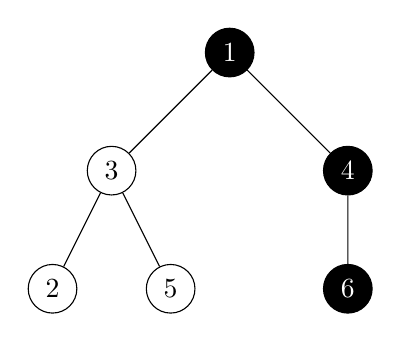
\begin{tikzpicture}[level/.style={sibling distance=30mm/#1}]
\node [circle,draw,fill=black,text=white] (1) {1}
  child { 
    node [circle,draw,fill=white] (3) {3}
    child { node [circle,draw,fill=white] (2) {2} }
    child { node [circle,draw,fill=white] (5) {5} }
  }
  child {
    node [circle,draw,fill=black,text=white] (4) {4}
    child { node [circle,draw,fill=black,text=white] (6) {6} }
  };
\end{tikzpicture}
\end{center}
\begin{itemize}
\item 节点颜色:\textcolor{red}{1(1)}, \textcolor{blue}{2(0)}, \textcolor{blue}{3(0)}, \textcolor{red}{4(1)}, \textcolor{blue}{5(0)}, \textcolor{red}{6(1)}
\item 颜色序列:\texttt{\textcolor{red}{1}\textcolor{blue}{0}\textcolor{blue}{0}\textcolor{red}{1}\textcolor{blue}{0}\textcolor{red}{1}}
\end{itemize}

\item \textbf{第一次操作(节点1)}:
\begin{center}
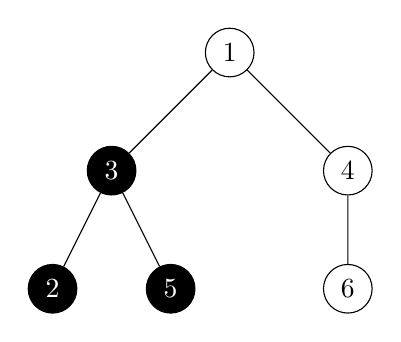
\begin{tikzpicture}[level/.style={sibling distance=30mm/#1}]
\node [circle,draw,fill=white] (1) {1}
  child { 
    node [circle,draw,fill=black,text=white] (3) {3}
    child { node [circle,draw,fill=black,text=white] (2) {2} }
    child { node [circle,draw,fill=black,text=white] (5) {5} }
  }
  child {
    node [circle,draw,fill=white] (4) {4}
    child { node [circle,draw,fill=white] (6) {6} }
  };
\end{tikzpicture}
\end{center}
\begin{itemize}
\item \textcolor{important}{\textbf{反转范围}}:\textcolor{orange}{整个树(所有节点)}
\item 反转后颜色:\textcolor{blue}{1(0)}, \textcolor{red}{2(1)}, \textcolor{red}{3(1)}, \textcolor{blue}{4(0)}, \textcolor{red}{5(1)}, \textcolor{blue}{6(0)}
\item 颜色序列:\texttt{\textcolor{blue}{0}\textcolor{red}{1}\textcolor{red}{1}\textcolor{blue}{0}\textcolor{red}{1}\textcolor{blue}{0}}
\end{itemize}

\item \textbf{第二次操作(节点3)}:
\begin{center}
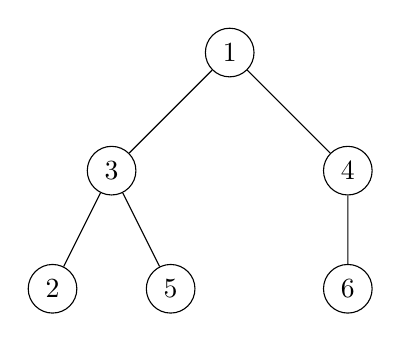
\begin{tikzpicture}[level/.style={sibling distance=30mm/#1}]
\node [circle,draw,fill=white] (1) {1}
  child { 
    node [circle,draw,fill=white] (3) {3}
    child { node [circle,draw,fill=white] (2) {2} }
    child { node [circle,draw,fill=white] (5) {5} }
  }
  child {
    node [circle,draw,fill=white] (4) {4}
    child { node [circle,draw,fill=white] (6) {6} }
  };
\end{tikzpicture}
\end{center}
\begin{itemize}
\item \textcolor{important}{\textbf{反转范围}}:\textcolor{orange}{节点3及其子树(节点3,2,5)}
\item 反转后颜色:\textcolor{blue}{1(0)}, \textcolor{blue}{2(0)}, \textcolor{blue}{3(0)}, \textcolor{blue}{4(0)}, \textcolor{blue}{5(0)}, \textcolor{blue}{6(0)}
\item 颜色序列:\texttt{\textcolor{blue}{0}\textcolor{blue}{0}\textcolor{blue}{0}\textcolor{blue}{0}\textcolor{blue}{0}\textcolor{blue}{0}}
\end{itemize}

\item \textbf{第三次操作(节点2)}:
\begin{center}
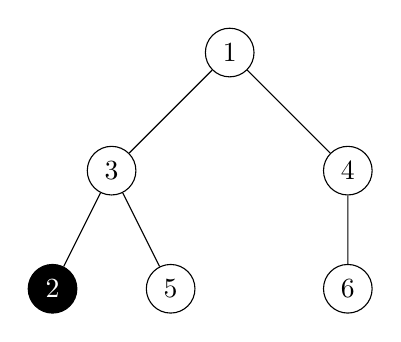
\begin{tikzpicture}[level/.style={sibling distance=30mm/#1}]
\node [circle,draw,fill=white] (1) {1}
  child { 
    node [circle,draw,fill=white] (3) {3}
    child { node [circle,draw,fill=black,text=white] (2) {2} }
    child { node [circle,draw,fill=white] (5) {5} }
  }
  child {
    node [circle,draw,fill=white] (4) {4}
    child { node [circle,draw,fill=white] (6) {6} }
  };
\end{tikzpicture}
\end{center}
\begin{itemize}
\item \textcolor{important}{\textbf{反转范围}}:\textcolor{orange}{节点2(只包含节点2)}
\item 反转后颜色:\textcolor{blue}{1(0)}, \textcolor{red}{2(1)}, \textcolor{blue}{3(0)}, \textcolor{blue}{4(0)}, \textcolor{blue}{5(0)}, \textcolor{blue}{6(0)}
\item 颜色序列:\texttt{\textcolor{blue}{0}\textcolor{red}{1}\textcolor{blue}{0}\textcolor{blue}{0}\textcolor{blue}{0}\textcolor{blue}{0}}
\end{itemize}
\end{enumerate}

\subsection*{背景知识}

在解决树结构相关问题时,图的存储方式至关重要。以下是两种常见的图存储方法:

\begin{enumerate}
\item \textcolor{highlight}{\textbf{邻接矩阵}}
\begin{itemize}
\item 使用二维数组 $graph[i][j]$ 表示节点 $i$ 到节点 $j$ 的边
\end{itemize}

\begin{lstlisting}[language=C++]
vector<vector<int>> graph(n + 1, vector<int>(n + 1, 0));
for (int i = 0; i < m; i++) {
    int u, v, w;
    cin >> u >> v >> w;
    graph[u][v] = w;
    graph[v][u] = w; 
}

\end{lstlisting}

\item \textcolor{highlight}{\textbf{邻接表}}
\begin{itemize}
\item 为每个节点维护一个链表,存储该节点的所有相连的节点
\end{itemize}

\begin{lstlisting}[language=C++]
vector<vector<int>> adj(n + 1);
for (int i = 0; i < m; i++) {
    int u, v;
    cin >> u >> v;
    adj[u].push_back(v);
    adj[v].push_back(u);
}
\end{lstlisting}

\item \textcolor{highlight}{\textbf{优缺点对比}}
\begin{table}[h]
\centering
\begin{tabularx}{\textwidth}{|l|X|X|X|X|X|}
\hline
\textbf{存储方式} & \textbf{空间复杂度} & \textbf{查询边(u,v)} & \textbf{遍历邻居} & \textbf{优点} & \textbf{缺点} \\
\hline
邻接矩阵 & $O(n^2)$ & $O(1)$ & $O(n)$ & \begin{tabular}[c]{@{}l@{}}查询速度快\\适合稠密图\end{tabular} & \begin{tabular}[c]{@{}l@{}}空间占用大\\不适合稀疏图\end{tabular} \\
\hline
邻接表 & $O(n+m)$ & $O(\text{deg}(u))$ & $O(\text{deg}(u))$ & \begin{tabular}[c]{@{}l@{}}空间效率高\\适合稀疏图\end{tabular} & \begin{tabular}[c]{@{}l@{}}查询边需遍历\\实现稍复杂\end{tabular} \\
\hline
\end{tabularx}
\end{table}
\end{enumerate}



\subsection*{算法分析}

\begin{enumerate}
\item \textcolor{highlight}{\textbf{直接模拟方法}}\\
对于每次操作,遍历以该节点为根的子树,反转所有节点的颜色 \par
这种方法的时间复杂度为 $O(n \cdot q)$,在 $n,q = 10^5$ 时会超时。

\item \textcolor{highlight}{\textbf{优化方法:标记传递}}\\
利用标记数组记录每个节点被反转的次数,最后统一处理。

\begin{enumerate}
\item \textcolor{highlight}{\textbf{核心思想}}
\begin{itemize}
\item 使用一个标记数组 \texttt{tag} 记录每个节点被反转的次数
\item 对于每次操作,只在操作节点上增加标记
\item 通过一次遍历,将父节点的标记传递给子节点
\item 如果反转次数是奇数,则反转当前节点, 否则不反转
\end{itemize}


\item \textcolor{highlight}{\textbf{算法步骤}}
\begin{itemize}
\item 构建二叉树结构(使用邻接表)
\item 初始化标记数组 \texttt{tag} 为 0
\item 对于每个操作,\texttt{tag[操作节点]++}
\item 使用 BFS 从根节点开始遍历,将父节点的标记累加到子节点
\begin{lstlisting}[language=C++]
queue<pair<int, int>> qu;  `// {当前节点, 父节点}`
qu.push({1, 0});
while (!qu.empty()) {
    int u = qu.front().first;
    int fa = qu.front().second;
    qu.pop();
    
    for (int v : adj[u]) {
        if (v == fa) continue;
        tag[v] += tag[u];
        qu.push({v, u});
    }
}
\end{lstlisting}

\item 计算每个节点的最终颜色
\begin{lstlisting}[language=C++]
for (int i = 1; i <= n; i++) {
    if (tag[i] % 2 == 1) { `// 反转颜色`
        color[i] = (color[i] == '0') ? '1' : '0';
    }
}
\end{lstlisting}

\end{itemize}
\end{enumerate}
\end{enumerate}


\subsection*{拓展思考}
\begin{itemize}
\item 如果颜色的数目修改为k种,且每次操作是将该节点及其子树颜色全部设置为x,那么算法该如何修改?
\item 如果树不是二叉树,而是多叉树,算法是否仍然适用?
\end{itemize}


\end{document}

